\section{Additional Experimental Results}
\label{app:additional-experiments}

This appendix reports two supplemental studies. The first compares AIRL and
behavior cloning as first-stage policy estimators inside GenPQR. The second
studies the many-action regime, where the number of actions grows while the
overall sample size is held fixed, so the effective anchor sample size for
DeepPQR decreases mechanically.

\paragraph{AIRL versus behavior cloning.}
Table~\ref{tab:app-airl-vs-bc} compares GenPQR with neural FQE under two sample
sizes. In these experiments, behavior cloning outperforms AIRL in both reward
recovery and held-out policy fit, while requiring essentially the same runtime.
This supports the modular interpretation of GenPQR: the identification step
does not require AIRL specifically, and a simpler classifier can be preferable
when behavior imitation is already well-conditioned.

\begin{table}[htb]
\centering
\caption{GenPQR with neural FQE under AIRL and behavior cloning policy estimation. Entries are mean $\pm$ 95\% confidence interval over 100 seeds.}
\label{tab:app-airl-vs-bc}
\scriptsize
\setlength{\tabcolsep}{4pt}
\begin{tabular}{llcccc}
\toprule
Setting & Method & MSE $\downarrow$ & Corr. $\uparrow$ & NLL $\downarrow$ & Time $\downarrow$ \\
\midrule
200 trajs / common anchor & GenPQR (AIRL, NN) & 0.71 $\pm$ 0.08 & 0.68 $\pm$ 0.03 & 1.648 $\pm$ 0.006 & 0.50 $\pm$ 0.01 \\
200 trajs / common anchor & GenPQR (BC, NN) & \textbf{0.54 $\pm$ 0.08} & \textbf{0.71 $\pm$ 0.02} & \textbf{1.616 $\pm$ 0.005} & 0.51 $\pm$ 0.01 \\
\midrule
1000 trajs / common anchor & GenPQR (AIRL, NN) & 0.63 $\pm$ 0.06 & 0.72 $\pm$ 0.02 & 1.606 $\pm$ 0.005 & 5.13 $\pm$ 0.34 \\
1000 trajs / common anchor & GenPQR (BC, NN) & \textbf{0.38 $\pm$ 0.06} & \textbf{0.81 $\pm$ 0.01} & \textbf{1.546 $\pm$ 0.004} & 5.18 $\pm$ 0.37 \\
\bottomrule
\end{tabular}
\end{table}

\paragraph{Many-action regime.}
Figure~\ref{fig:app-many-action} fixes the overall sample size at the
high-sample matched setting and increases the number of actions. As
\(|\mathcal A|\) grows, the effective anchor sample size falls from roughly
\(6400\) anchor-action transitions at \(|\mathcal A|=5\) to roughly \(800\) at
\(|\mathcal A|=40\). In this regime, DeepPQR degrades sharply, whereas GenPQR
remains substantially more stable because its \(Q\)-evaluation step continues
to use the full sample. We show both AIRL- and BC-based versions of each
method. Because this fixed-sample action-scaling study was run as a quick pilot
to validate the trend, the figure should be interpreted as directional.

\begin{figure*}[htb]
\centering
\begin{minipage}[c]{0.48\textwidth}
\centering
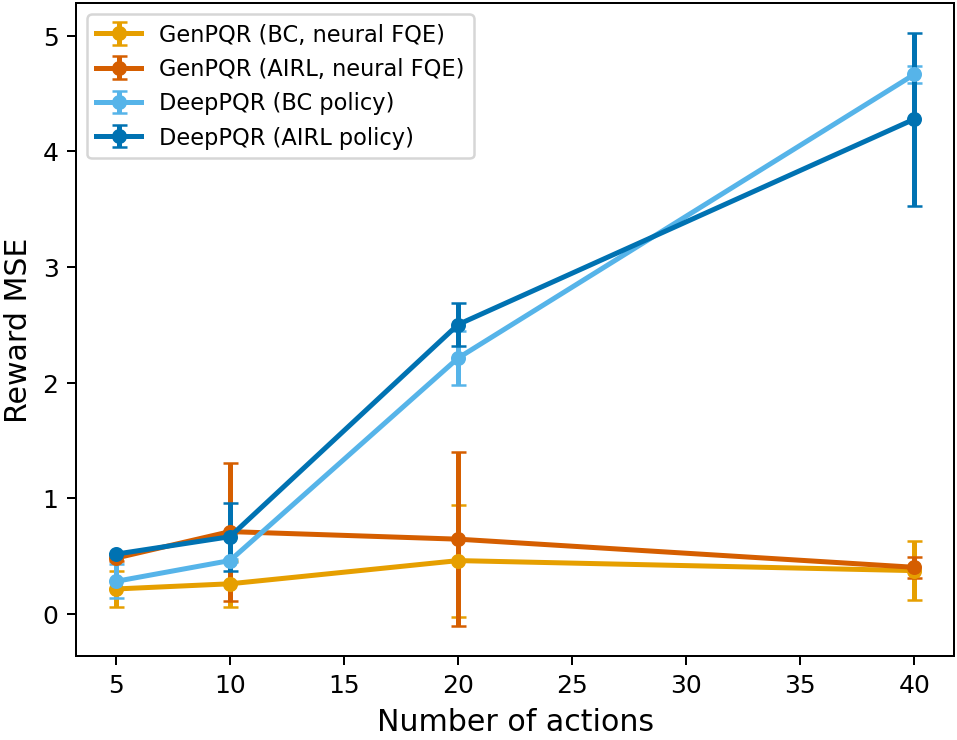
\includegraphics[width=\linewidth]{many_action_reward_mse.png}
\end{minipage}
\hfill
\begin{minipage}[c]{0.48\textwidth}
\centering
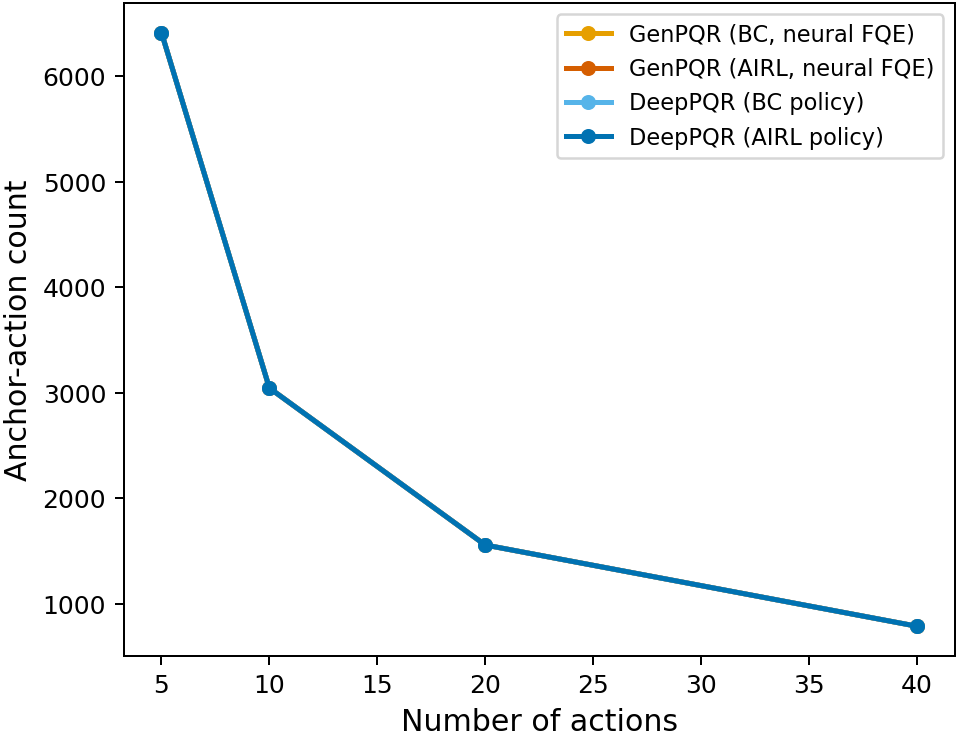
\includegraphics[width=\linewidth]{many_action_anchor_count.png}
\end{minipage}
\caption{Fixed-sample many-action study. Left: reward MSE as the number of actions increases. Right: realized anchor-action count over the same sweep. The total sample size is held fixed, so DeepPQR's effective sample size shrinks with \(|\mathcal A|\) while GenPQR continues to use the full sample in its \(Q\)-evaluation step.}
\label{fig:app-many-action}
\end{figure*}
